% This file was created by matplotlib v0.1.0.
% Copyright (c) 2010--2014, Nico Schlömer <nico.schloemer@gmail.com>
% All rights reserved.
% 
% The lastest updates can be retrieved from
% 
% https://github.com/nschloe/matplotlib2tikz
% 
% where you can also submit bug reports and leavecomments.
% 
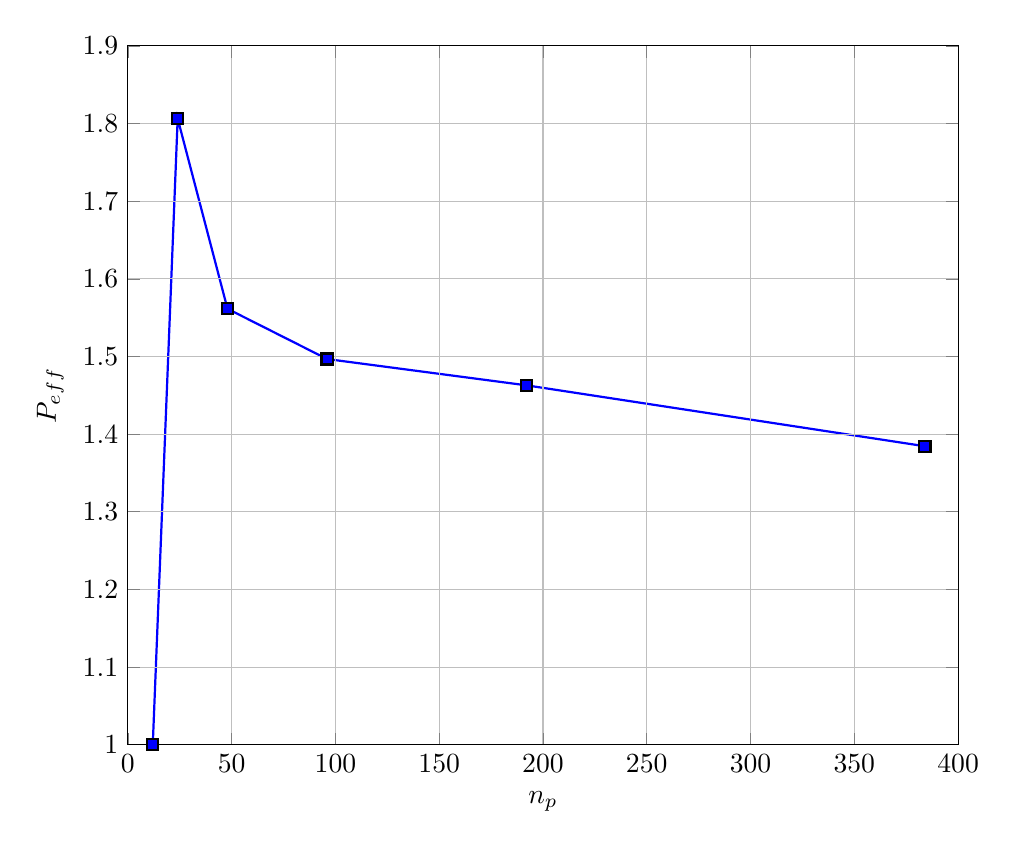
\begin{tikzpicture}

\begin{axis}[
xlabel={$n_p$},
ylabel={$P_{eff}$},
xmin=0, xmax=400,
ymin=1, ymax=1.9,
axis on top,
width=\textwidth,
xmajorgrids,
ymajorgrids
]
\addplot [thick, blue, mark=square*, mark size=2, mark options={draw=black}]
coordinates {
(12,1)
(24,1.80626410146194)
(48,1.56136430327869)
(96,1.49665918033873)
(192,1.46283025896665)
(384,1.38440521579281)

};
\path [draw=black, fill opacity=0] (axis cs:1,13)--(axis cs:1,13);

\path [draw=black, fill opacity=0] (axis cs:13,0)--(axis cs:13,0);

\path [draw=black, fill opacity=0] (axis cs:13,1)--(axis cs:13,1);

\path [draw=black, fill opacity=0] (axis cs:0,13)--(axis cs:0,13);

\end{axis}

\end{tikzpicture}